\documentclass[11pt,letterpaper]{article}
\usepackage[utf8]{inputenc}
\usepackage[spanish,es-noshorthands]{babel}
\usepackage[T1]{fontenc}
\usepackage{times}
\usepackage[margin=2.5cm]{geometry}
\usepackage{tikz}
\usetikzlibrary{shapes,arrows.meta,positioning,fit,backgrounds,shapes.multipart,calc}
\usepackage{booktabs}
\usepackage{longtable}
\usepackage{array}
\usepackage{xcolor}
\usepackage{hyperref}
\usepackage{enumitem}
\usepackage{graphicx}
\hypersetup{colorlinks=true,linkcolor=black,urlcolor=blue}

\begin{document}

\begin{titlepage}
\centering
{\LARGE \textbf{Universidad Técnica Estatal de Quevedo}}\\[0.5cm]


\includegraphics[width=2cm]{figs/logo_uteq.png}\\[0.5cm]

{\large \textbf{Facultad de Ciencias de la Computación}}\\[0.4cm]

{\large \textbf{Asignatura:}} Ingeniería De Requerimientos\\[0.3cm]

{\large \textbf{Estudiante:}} Huilcapi Leon Denisses Fabiola\\[0.3cm]

{\large \textbf{Curso:}} 4to ``A''\\[0.3cm]

{\large \textbf{Docente:}} Ing. Guerrero Ulloa Gleiston Ciceron\\[0.3cm]

{\large \textbf{URL:}} \url{https://github.com/huilcapi/Huilcapi_Evaluacion_UnidadIV}\\[0.6cm]

{\large \textbf{Resumen:}}\\[0.2cm]

\includegraphics[width=0.9\textwidth]{figs/resumen_sga.png}\\[0.6cm]

{\large \textbf{Evaluación:}}\\[0.2cm]
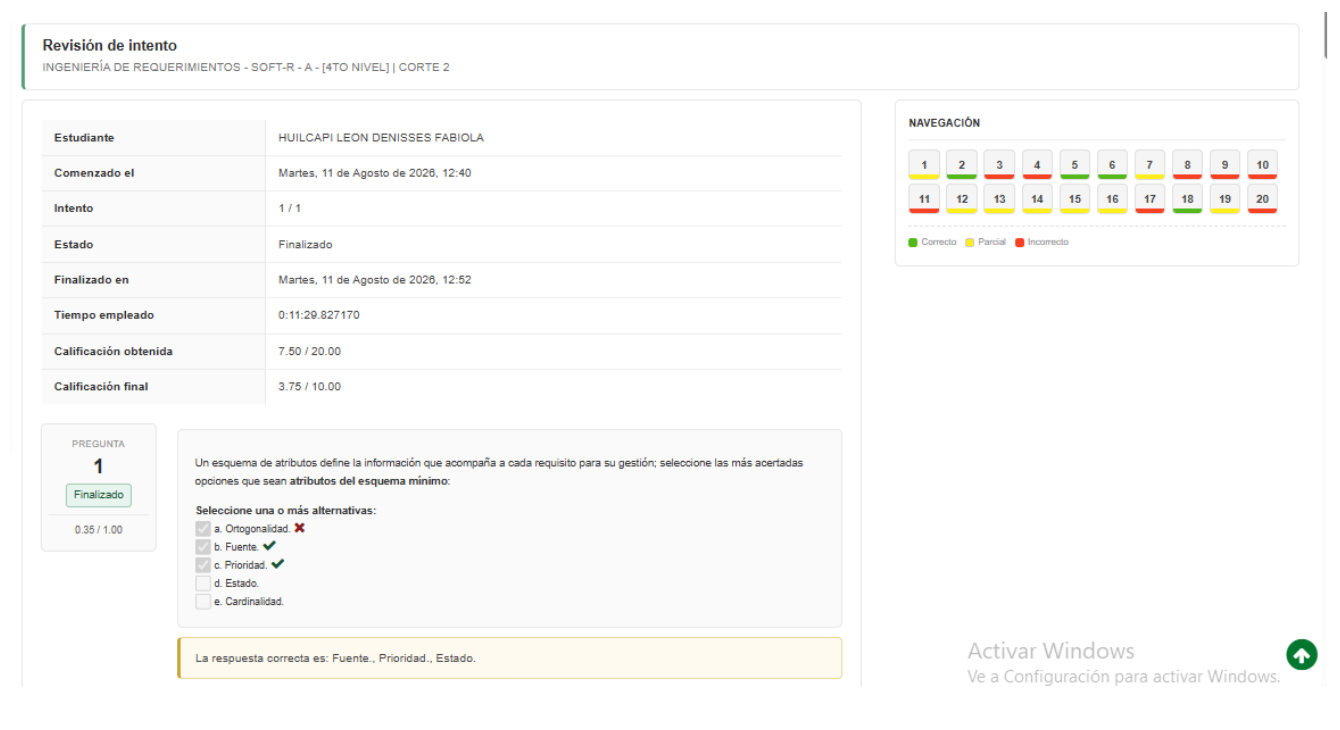
\includegraphics[width=0.78\textwidth]{figs/evaluacion_sga.png}

\end{titlepage}
\setcounter{page}{1}


\section*{Caso práctico}
Sistema de Gestión de Pedidos: un \textbf{Cliente} (cédula/RUC, nombre, correo) realiza cero o más \textbf{Pedidos}. Cada \textbf{Pedido} (identificador, fecha, total) contiene una o más \textbf{Líneas de pedido}, y cada línea referencia un \textbf{Producto} (código, descripción, precio, stock). Al registrar un pedido se verifica stock: si hay existencias se confirma; si no, se notifica el faltante. Un pedido confirmado puede despacharse, luego entregarse, o anularse mientras no haya sido entregado.

% ============================================================
\section{P1. Modelo de datos --- Diagrama de clases UML}

\begin{center}
\begin{tikzpicture}[
  class/.style={rectangle split, rectangle split parts=3, draw=black, thick,
    rectangle split part align=left, text width=4.6cm, font=\footnotesize},
  every node/.style={align=left}
]

\node[class] (cliente) at (0,0) {
  \centering\textbf{Cliente}
  \nodepart{second}
  \underline{cedulaRUC: Integer}\\
  nombre: String\\
  correo: String
  \nodepart{third}
  + registrarPedido(p: Pedido): void\\
  + consultarPedido(): List$\langle$Pedido$\rangle$
};

\node[class, right=4.7cm of cliente] (pedido) {
  \centering\textbf{Pedido}
  \nodepart{second}
  \underline{idPedido: Integer}\\
  fecha: DateTime\\
  total: Decimal\\
  estado: EstadoPedido
  \nodepart{third}
  + confirmar(): void\\
  + despachar(): void\\
  + entregar(): void\\
  + anular(): void\\
  + calcularTotal(): Decimal
};

\node[class, below=1.6cm of pedido] (linea) {
  \centering\textbf{LineaPedido}
  \nodepart{second}
  \underline{numLinea: Integer}\\
  cantidad: Integer\\
  precioUnitario: Decimal
  \nodepart{third}
  + calcularSubtotal(): Decimal
};

\node[class, below=1.6cm of cliente] (producto) {
  \centering\textbf{Producto}
  \nodepart{second}
  \underline{codigo: Integer}\\
  descripcion: String\\
  precio: Decimal\\
  stock: Integer
  \nodepart{third}
  + verificarDisponibilidad(c: Integer): boolean\\
  + DescontarStock(c: Integer): void
};

\draw[-] (cliente) -- (pedido) node[midway, above, font=\scriptsize] {realiza};
\node[font=\scriptsize] at ($(cliente.east)+(0.6,0.28)$) {1};
\node[font=\scriptsize] at ($(pedido.west)+(-0.6,0.28)$) {0..*};

\draw[-] (pedido) -- (linea) node[midway, right, font=\scriptsize] {contiene};
\node[font=\scriptsize] at ($(pedido.south)+(-0.3,-0.15)$) {1};
\node[font=\scriptsize] at ($(linea.north)+(-0.3,0.15)$) {0..*};

\draw[-] (linea) -- (producto) node[midway, above, font=\scriptsize] {};
\node[font=\scriptsize] at ($(linea.west)+(-0.6,0.28)$) {0..*};
\node[font=\scriptsize] at ($(producto.east)+(0.6,0.28)$) {1};

\end{tikzpicture}
\end{center}
% ============================================================
\section{P2. Modelo funcional --- Diagrama de actividades UML: ``Registrar pedido''}

\begin{center}
\begin{tikzpicture}[
  action/.style={rectangle, draw=black, thick, minimum width=3cm, minimum height=0.9cm, align=center, font=\footnotesize, fill=white},
  decision/.style={diamond, draw=black, thick, aspect=2.4, minimum width=2.6cm, align=center, font=\footnotesize, fill=white},
  >=Stealth
]

% --- Marco y carriles (swimlanes) ---
\draw[thick] (0,0) rectangle (9,10.2);
\draw[thick] (4.4,0) -- (4.4,9.5);
\draw[thick] (0,9.5) -- (9,9.5);
\node[font=\bfseries] at (4.5,9.9) {Registrar pedido};
\node[font=\bfseries\footnotesize] at (2.2,9.15) {Cliente};
\node[font=\bfseries\footnotesize] at (6.7,9.15) {Sistema};

% --- Nodos ---
\node[circle, draw=black, fill=black, minimum size=0.3cm] (start) at (2.2,8.6) {};
\node[action] (ingresar) at (2.2,7.6) {Ingresar datos\\del pedido};
\node[action] (verificar) at (2.2,6.4) {Verificar disponi-\\bilidad de stock};
\node[decision] (dec) at (2.2,5.0) {¿Stock\\disponible?};
\node[action] (confirmar) at (2.2,3.6) {Confirmar el pedido};
\node[action, minimum width=4.2cm] (registrar) at (2.7,2.2) {Registrar resultado y\\notificar cliente};
\node[action] (notificar) at (6.7,5.0) {Notificar\\faltante};
\node[circle, draw=black, thick, minimum size=0.35cm] (endc) at (2.7,1.0) {};
\node[circle, draw=black, fill=black, minimum size=0.18cm] at (endc) {};

% --- Flujo ---
\draw[->] (start) -- (ingresar);
\draw[->] (ingresar) -- (verificar);
\draw[->] (verificar) -- (dec);
\draw[->] (dec) -- node[left, font=\scriptsize] {sí} (confirmar);
\draw[->] (dec.east) -- node[above, font=\scriptsize] {no} (notificar.west);
\draw[->] (confirmar) -- (registrar);
\draw[->] (notificar.south) |- (registrar.east);
\draw[->] (registrar) -- (endc);

\end{tikzpicture}
\end{center}
% ============================================================
\section{P3. Modelo de comportamiento --- Máquina de estados UML del Pedido}

\begin{center}
\begin{tikzpicture}[
  state/.style={rectangle, rounded corners, draw=black, thick, minimum width=2.6cm, minimum height=0.9cm, align=center, font=\footnotesize},
  initial/.style={circle, draw=black, fill=black, minimum size=0.3cm},
  final/.style={circle, draw=black, thick, minimum size=0.35cm},
  >=Stealth
]
\node[initial] (i) at (0,0) {};
\node[state, right=1.3cm of i] (reg) {Registrado};

\begin{scope}[on background layer]
\node[draw=black, dashed, thick, rounded corners, fit=(reg), inner sep=0pt] {};
\end{scope}

\node[state, right=2.3cm of reg] (conf) {Confirmado};
\node[state, right=2.3cm of conf] (env) {Enviado};
\node[state, below right=1.6cm and -0.3cm of env] (ent) {Entregado};
\node[final, right=0.7cm of ent] (fin) {};
\node[circle, draw=black, fill=black, minimum size=0.18cm] at (fin) {};

\node[state, below=2.4cm of conf] (canc) {Cancelado};

% superestado que agrupa Registrado, Confirmado, Enviado
\node[draw=black, dashed, thick, rounded corners, fit=(reg)(conf)(env), inner sep=0.35cm] (super) {};
\node[font=\scriptsize, above=1pt of super.north] {Activo (superestado)};

\draw[->] (i) -- (reg);
\draw[->] (reg) -- node[above, font=\scriptsize, align=center] {confirmarPedido()\\ (stock disponible)} (conf);
\draw[->] (conf) -- node[above, font=\scriptsize] {despachar()} (env);
\draw[->] (env) -- node[above right, font=\scriptsize] {entregar()} (ent);
\draw[->] (ent) -- (fin);
\draw[->] (super.south) -- node[right, font=\scriptsize, align=left] {anular()\\ (no entregado)} (canc);
\end{tikzpicture}
\end{center}
% ============================================================
\section{P4. Consistencia entre las tres perspectivas}

\begin{center}
\small
\begin{tabular}{p{2.2cm}p{3.8cm}p{4.8cm}p{2.8cm}}
\toprule
\textbf{Evento (P3)} & \textbf{Función/acción (P2)} & \textbf{Entidad/atributo (P1)} & \textbf{Observación} \\
\midrule
confirmarPedido() & Confirmar pedido & Pedido.estado, Pedido.confirmar() & Consistente \\
despachar() & (no modelado en P2, fuera de alcance de ``Registrar pedido'') & Pedido.estado, Pedido.despachar() & Consistente por alcance \\
entregar() & (no modelado en P2) & Pedido.estado, Pedido.entregar() & Consistente por alcance \\
anular() & (no modelado en P2) & Pedido.estado, Pedido.anular() & Consistente \\
\bottomrule
\end{tabular}
\end{center}
% ============================================================
\section{P5. Especificación de requisitos con esquema de atributos}

\subsection*{RF-01 (Funcional)}
\begin{center}\small
\begin{tabular}{lp{10.5cm}}
\toprule
\textbf{Atributo} & \textbf{Valor} \\
\midrule
Identificador & RF-01 \\
Descripción & El sistema debe permitir registrar un pedido verificando la disponibilidad de stock de cada producto antes de confirmarlo. \\
Prioridad & Alta \\
Estado & Propuesto \\
Fuente & Caso de negocio --- Sistema de Gestión de Pedidos \\
Estabilidad & Estable \\
Versión & 1.0 \\
Método de verificación & Prueba funcional (caso de prueba) \\
\bottomrule
\end{tabular}
\end{center}

\subsection*{RF-02 (Funcional)}
\begin{center}\small
\begin{tabular}{lp{10.5cm}}
\toprule
\textbf{Atributo} & \textbf{Valor} \\
\midrule
Identificador & RF-02 \\
Descripción & El sistema debe permitir anular un pedido confirmado o enviado siempre que no haya sido entregado. \\
Prioridad & Media \\
Estado & Propuesto \\
Fuente & Caso de negocio --- Sistema de Gestión de Pedidos \\
Estabilidad & Estable \\
Versión & 1.0 \\
Método de verificación & Prueba funcional (caso de prueba) \\
\bottomrule
\end{tabular}
\end{center}

\subsection*{RNF-01 (No funcional --- ISO/IEC 25010:2023, Eficiencia de desempeño)}
\begin{center}\small
\begin{tabular}{lp{10.5cm}}
\toprule
\textbf{Atributo} & \textbf{Valor} \\
\midrule
Identificador & RNF-01 \\
Descripción & El sistema debe registrar un pedido en menos de 3 segundos, medido desde el envío del formulario hasta la confirmación en pantalla, bajo carga de 50 usuarios concurrentes. \\
Característica 25010 & Eficiencia de desempeño (tiempo de respuesta) \\
Métrica / umbral & Tiempo de respuesta $<$ 3 s (percentil 95) \\
Prioridad & Alta \\
Estado & Propuesto \\
Fuente & Requisito de negocio (``registrar pedidos con rapidez'') \\
Estabilidad & Estable \\
Versión & 1.0 \\
Método de verificación & Prueba de rendimiento (carga) \\
\bottomrule
\end{tabular}
\end{center}

\subsection*{RNF-02 (No funcional --- ISO/IEC 25010:2023, Seguridad)}
\begin{center}\small
\begin{tabular}{lp{10.5cm}}
\toprule
\textbf{Atributo} & \textbf{Valor} \\
\midrule
Identificador & RNF-02 \\
Descripción & El sistema debe proteger los datos personales del cliente (cédula/RUC, nombre, correo) cifrándolos en reposo con AES-256 y restringiendo su acceso a usuarios autorizados. \\
Característica 25010 & Seguridad (confidencialidad) \\
Métrica / umbral & 100\% de los campos personales cifrados; 0 accesos no autorizados registrados en auditoría \\
Prioridad & Alta \\
Estado & Propuesto \\
Fuente & Requisito de negocio (``proteger los datos personales del cliente'') \\
Estabilidad & Estable \\
Versión & 1.0 \\
Método de verificación & Inspección de configuración / prueba de seguridad \\
\bottomrule
\end{tabular}
\end{center}

% ============================================================
\section{P6. Priorización MoSCoW}

\begin{center}\small
\begin{tabular}{lll p{6.5cm}}
\toprule
\textbf{Req.} & \textbf{Categoría} & \textbf{Valor/Viabilidad} & \textbf{Justificación} \\
\midrule
RF-01 & Must have & Alto valor, alta viabilidad & Sin verificación de stock el sistema no cumple su propósito central; es viable con la tecnología disponible. \\
RNF-02 & Must have & Alto valor, viabilidad media & La protección de datos personales es obligatoria legal y contractualmente; es exigible desde el primer incremento. \\
RF-02 & Should have & Valor medio-alto, alta viabilidad & Importante para el ciclo de vida del pedido, pero el sistema puede operar en un primer incremento sin anulación automática (proceso manual temporal). \\
RNF-01 & Could have & Valor medio, viabilidad media & Mejora la experiencia, pero el sistema es funcional aunque el tiempo de respuesta supere el umbral en una primera versión. \\
\bottomrule
\end{tabular}
\end{center}

% ============================================================
\section{P7. Validación por inspección (checklist ISO/IEC/IEEE 29148)}

\subsection*{Paso 1 --- Identificación de defectos (sin corregir)}
\begin{center}\small
\begin{tabular}{lp{2.2cm}p{7.8cm}}
\toprule
\textbf{Req.} & \textbf{Propiedad violada} & \textbf{Defecto detectado} \\
\midrule
RF-02 & No ambiguo & ``siempre que no haya sido entregado'' no aclara qué ocurre si el pedido ya está \texttt{Cancelado}; term. ambiguo sobre estados válidos de origen. \\
RNF-01 & Verificable & ``bajo carga de 50 usuarios concurrentes'' no especifica el perfil de carga (tipo de operación, duración de la prueba), dificultando la verificación exacta. \\
RF-01 & Singular & Combina dos capacidades (verificar stock \emph{y} confirmar el pedido) en un solo enunciado, lo que dificulta trazar pruebas independientes. \\
\bottomrule
\end{tabular}
\end{center}

\subsection*{Paso 2 --- Retrabajo (requisitos corregidos)}
\begin{center}\small
\begin{tabular}{lp{11cm}}
\toprule
\textbf{Req.} & \textbf{Redacción corregida} \\
\midrule
RF-02 & El sistema debe permitir anular un pedido que se encuentre en estado \texttt{Registrado}, \texttt{Confirmado} o \texttt{Enviado}; la operación debe rechazarse si el pedido está en estado \texttt{Entregado} o \texttt{Cancelado}. \\
RNF-01 & El sistema debe registrar un pedido en menos de 3 segundos (percentil 95), medido en una prueba de carga con 50 usuarios ejecutando la operación ``registrar pedido'' de forma concurrente durante 10 minutos. \\
RF-01 & (Dividido en dos) RF-01a: El sistema debe verificar la disponibilidad de stock de cada producto de un pedido antes de confirmarlo. RF-01b: El sistema debe confirmar el pedido únicamente cuando exista stock suficiente para todas sus líneas. \\
\bottomrule
\end{tabular}
\end{center}


\end{document}
